%!TEX program = xelatex
\documentclass[table,aspectratio=169]{beamer}

%\usefonttheme{professionalfonts}
\usepackage[T1]{fontenc}
\renewcommand*\familydefault{\sfdefault}

\usepackage{beamerthemesplit}
\usepackage{graphicx}
\graphicspath{{./Figures/}}

\usepackage{bm,bbm,bbding}
\usepackage{natbib}
\usepackage{siunitx}
\usepackage{texnames}
\usepackage{algorithm,algpseudocode}
\usepackage{multirow}
\usepackage{booktabs}
\usepackage{amsmath}
\usepackage{mathabx}
\usepackage{scalerel,stackengine}
\stackMath
\newcommand\reallywidehat[1]{%
	\savestack{\tmpbox}{\stretchto{%
			\scaleto{%
				\scalerel*[\widthof{\ensuremath{#1}}]{\kern-.6pt\bigwedge\kern-.6pt}%
				{\rule[-\textheight/2]{1ex}{\textheight}}%WIDTH-LIMITED BIG WEDGE
			}{\textheight}% 
		}{0.5ex}}%
	\stackon[1pt]{#1}{\tmpbox}%
}
\parskip 1ex

\definecolor{anti-flashwhite}{rgb}{0.95, 0.95, 0.96}
\definecolor{byzantine}{rgb}{0.74, 0.2, 0.64}
\definecolor{VUWlightgreen}{rgb}{0, .294, .204}
\definecolor{VUWgreen}{rgb}{0, .196, .136}

\usetheme[numbering=fraction]{metropolis}

\setbeamercovered{dynamic}
\setbeamercolor{background canvas}{bg=VUWgreen}
\setbeamercolor{normal text}{fg=anti-flashwhite, bg=VUWgreen}
\setbeamercolor{frametitle}{bg=VUWlightgreen,fg=anti-flashwhite}
\setbeamercolor{footline}{bg=VUWlightgreen}

\makeatletter
\setlength{\metropolis@frametitle@padding}{.5em}% <- default 2.2 ex

\setbeamertemplate{footline}{%
\begin{beamercolorbox}[wd=\textwidth, sep=.2ex]{footline}% <- default 3ex
\usebeamerfont{page number in head/foot}%
\usebeamertemplate*{frame footer}
\hfill%
\usebeamertemplate*{frame numbering}
\end{beamercolorbox}%
}
\makeatother

\setbeamertemplate{frame footer}{\includegraphics[width=1.5cm]{"Logo Offshore Reversed Landscape RGB"}}
\setbeamertemplate{navigation symbols}{}

\AtBeginSubsection[]
{
\begin{frame}
\frametitle{Table of Contents}
\tableofcontents[currentsection,currentsubsection]
\end{frame}
}

\title{Identifying Heterogeneity in SAR Data with New Test Statistics}
\subtitle{No problem is too old, and you don't always need deep learning}
\author{Alejandro C.\ Frery}
\institute{Victoria University of Wellington\\
School of Mathematics and Statistics\\
New Zealand}
\date{November, 2024}

\begin{document}

\setsansfont[BoldFont={Avenir Heavy}]{Avenir Book}

\frame{\titlepage}

\begin{frame}
This is a joint work with Prof.\ Abraão Nascimento and MSc.\ Janeth Alpala (it is part of her PhD project), from Universidade Federal de Pernambuco, Brazil.
\end{frame}

\begin{frame}{Starting point}
\begin{itemize}[<+->]
	\item Synthetic Aperture Radar (SAR) technology is essential for environmental monitoring and disaster management. 
	\item It provides
	images under various conditions, including day or night and adverse weather
	situations~\citep{Moreira2013,Mu2019}. 
	\item The effective use of SAR
	data relies on understanding of their statistical properties
	because it is corrupted by speckle: a noise-like interference effect~\citep{Argenti2013}.
	\item Speckle in intensity format is non-Gaussian. 
	\item The
	\({G}^0\) distribution is suitable for SAR data and includes
	the Gamma law as the limiting case for fully-developed
	speckle~\citep{Ferreira2020}.
	\item We improve the identification of potential roughness
	features in SAR intensity data, i.e., departures from the Gamma distribution (fully-developed
	speckle).
\end{itemize}
\end{frame}

\begin{frame}{The problem}
\centering
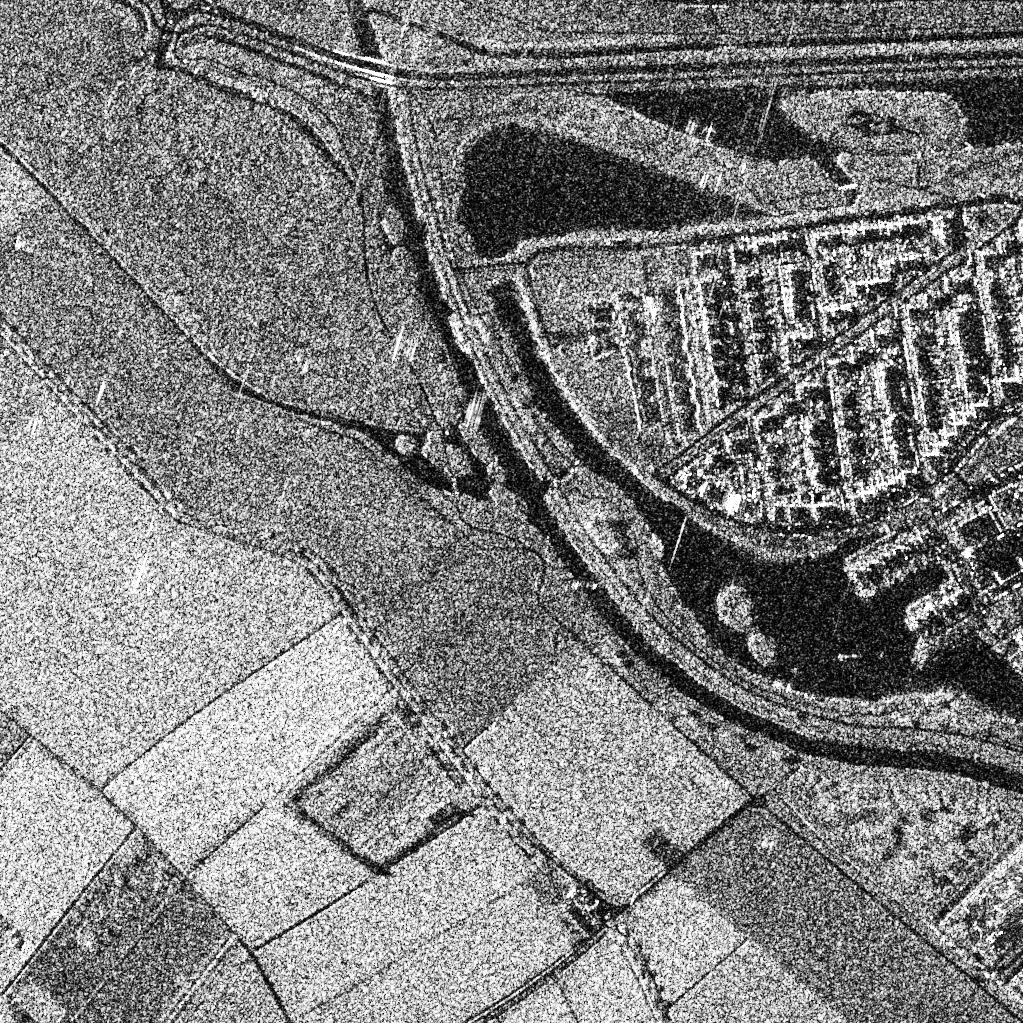
\includegraphics[width=55mm]{../Figures/PNG/Rotterdam_1024}\hskip1em
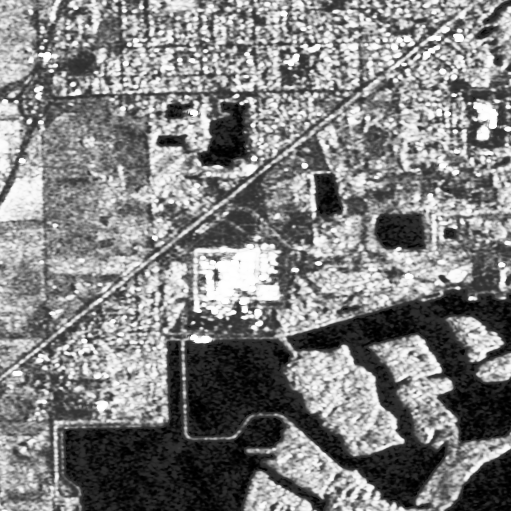
\includegraphics[width=55mm]{../Figures/PNG/lake_512}

Apart from the brightness, notice that different types of areas have distinct roughness.
\end{frame}

\begin{frame}[allowframebreaks]{Statistical models}
The main models are the Gamma (suitable for fully-developed speckle) and
\({G}_I^0\) (able to describe roughness) distributions~\citep{Frery1997}. 

They are characterized by the probability
density functions (pdfs): 
\begin{align}
	f_Z(z;L, \mu\mid \Gamma_{\text{SAR}})&=\frac{L^L}{\Gamma(L)\mu^L}z^{L-1}\exp\left\{-Lz/\mu\right\} \mathbbm 1_{\mathbbm R_+}(z)\label{E:gamma1}\\
	\intertext{ and }
	f_Z\big(z; \mu, \alpha, L\mid G_I^0\big) &= \frac{L^L\Gamma(L-\alpha)}{\big[-\mu(\alpha+1)\big]^{\alpha}\Gamma(-\alpha)\Gamma(L)} \frac{z^{L-1}}{\big[-\mu(\alpha+1)+Lz\big]^{L-\alpha}}\mathbbm 1_{\mathbbm R_+}(z),\label{E:gi01}
\end{align} 
where \(\mu > 0\) is the mean,
\(\alpha < 0\) measures the roughness, \(L \geq 1\) is the number of
looks, \(\Gamma(\cdot)\) is the gamma function, and
\(\mathbbm 1_{A}(z)\) is the indicator function of the set \(A\).

\citet{Frery1997} proved that the $\Gamma_{\text{SAR}}$ model is a particular case of the $G_I^0$ distribution.
In effect, for a given $\mu$ fixed,
$$
f_Z\big(z; \mu, \alpha, L\mid G_I^0\big)
\longrightarrow 
f_Z(z;L, \mu\mid \Gamma_{\text{SAR}}) 
$$
when $\alpha\to-\infty$.
\end{frame}

\begin{frame}{The statistical approach}
\begin{columns}
	\begin{column}{.63\linewidth}
{\includegraphics<1>[width=\linewidth]{../Figures/PDF/GammaGI0Densities}}
{\includegraphics<2>[width=\linewidth]{../Figures/PDF/GammaGI0DensitiesSemilog}}
	\end{column}
	\begin{column}{.3\linewidth}
	We need to identify the model that best describes the data.
	
	But it is a challenging task because
	\begin{itemize}
		\item Samples are small, and
		\item Parameter estimators are tricky.
	\end{itemize}
	\end{column}
\end{columns}
\end{frame}

\begin{frame}{The usual approach: I}
Assume the equivalent number of looks $L$ is known.

The coefficient of variation under the $\Gamma_{\text{SAR}}$ models is:
\begin{align}
	\text{CV}\mid \Gamma_{\text{SAR}} =
	\frac{\sigma}{\mu} =
	 \frac{1}{\sqrt{L}}.
\end{align}

Procedure:
\begin{enumerate}
	\item Collect (typically small) samples $\bm x_1, \bm x_2, \dots, \bm x_m$.
	\item Compute the sample coefficients of variation $\text{CV}(\bm x_1),\text{CV}(\bm x_2), \dots, \text{CV}(\bm x_m)$.
	\item Decide for heterogeneity those samples ``too far'' from $1/\sqrt{L}$.
\end{enumerate}

But, what is ``too far''?
\end{frame}


\begin{frame}{The usual approach: I}
We are tempted to form a statistical test using the coefficient of variation as the test statistic.

Consider the random sample $\bm X=(X_1,X_2,\dots,X_n)$ that, under the null hypothesis has $\Gamma_{\text{SAR}}$ distribution.
Then, we need the distribution of
\begin{equation}
\widehat{\text{CV}}(\bm X) = \frac{\frac1n \sum_{\ell=1}^n X_\ell}{\sqrt{\frac1n \sum_{\ell=1}^n \big(X_\ell-\overline{\bm X}\big)^2}}.
\label{eq:CV}
\end{equation}

Although we know that $\bar{\bm X}$ and $\widehat{\text{CV}}(\overline X) $ are independent \citep{OnaCharacterizationoftheGammaDistributiontheIndependenceoftheSampleMeanandtheSampleCoefficientofVariation}, we don't know the distribution of~\eqref{eq:CV}.
\end{frame}

\begin{frame}{The usual approach: II}
The coefficient of variation is so widespread that \citet{Ospina2019} proposed alternative ways of computing it.

They replaced the mean by the median, and the standard deviation by the mean absolute deviation from the median (MnAD), two well-known robust measures of location and 
scale, respectively. 

Their estimator becomes
\begin{equation}
\widecheck{\text{CV}}(\bm X) = \frac{\widehat{Q}_2(\bm X)}{\frac1n \sum_{\ell=1}^n|X_i-\widehat{Q}_2(\bm X)|}.
\end{equation}

It is robust, we don't know its distribution under the $\Gamma_{\text{SAR}}$ model.
\end{frame}

\begin{frame}[allowframebreaks]{Our proposal's rationale}
The entropy is a powerful descriptor.
It has been used for SAR data, among others, by
\citet{Ferreira2020} for segmentation, by
\citet{Cassetti2022} for classification, and by 
\citet{EntropyBasedNonLocalMeansFilterforSingleLookSARSpeckleReduction} for noise reduction.

Specifically, the Shannon entropy of the model $F$, characterized by the probability density function $f$ is
$$
H(F) = -\int f(x) \ln\big(f(x)\big) dx.
$$

There are other types of entropy, e.g., Rényi and Tsallis, and also the Fisher information measure~\citep{AsymptoticDistributionofCertainTypesofEntropyundertheMultinomialLaw}.
These quantities have not been explored for roughness assessment (\alert{hint!}).

The Shannon entropy of
\(\Gamma_{\text{SAR}}\) in~\eqref{E:gamma1} and \(G_I^0\) 
in~\eqref{E:gi01}: 
\begin{equation}
	\label{E:E-gamma}
	H_{\Gamma_{\text{SAR}}}(L, \mu) =   L -\ln L+\ln\Gamma(L)+(1-L)\psi^{(0)}(L) + \ln \mu, 
\end{equation} \begin{multline}
	\label{E:E-GIO}
	H_{G_I^0}(\mu, \alpha, L) =L -\ln L+\ln\Gamma(L)+(1-L)\psi^{(0)}(L) +\ln \mu -\ln\Gamma(L-\alpha)\\
	+ (L-\alpha) \psi^{(0)}(L-\alpha)-(1-\alpha)\psi^{(0)}(-\alpha)+\ln (-1-\alpha)+\ln\Gamma(-\alpha)-L,
\end{multline} where \(\psi^{(0)}(\cdot)\) is the digamma function.

\alert{They are different! Check \citet{IdentifyingHeterogeneityinSARDatawithNewTestStatistics} for details.} Therefore, some empirical version of~\eqref{E:E-gamma} could be used to form a test statistic.

Now, assume that we have a good estimator for the Shannon entropy, say $\widehat{H_{\Gamma_{\text{SAR}}}}$.
Under the $\Gamma_{\text{SAR}}$ model, we expect it to be close to~\eqref{E:E-gamma}.
Such estimator estimates
$$
\widehat{H_{\Gamma_{\text{SAR}}}} = \reallywidehat{L -\ln L+\ln\Gamma(L)+(1-L)\psi^{(0)}(L) + \ln \mu}
$$

Now we build a test statistic:
\begin{align*}
	S(\bm Z; L) = & \hskip1ex\reallywidehat{L -\ln L+\ln\Gamma(L)+(1-L)\psi^{(0)}(L) + \ln \mu} - \mbox{}\\
	& \hskip1ex L + \ln L - \ln\Gamma(L) - (1-L)\psi^{(0)}(L) - \ln \widehat{\mu}\\
	= & \hskip1ex \widehat{H_{\Gamma_{\text{SAR}}}} - L + \ln L - \ln\Gamma(L) - (1-L)\psi^{(0)}(L) - \ln \widehat{\mu}.
\end{align*}
This test statistic is close to zero under the null hypothesis (homogeneity, fully developed speckle, the $\Gamma_{\text{SAR}}$ model).

Now we must choose suitable estimators $\widehat{H_{\Gamma_{\text{SAR}}}}$ and $\widehat{\mu}$.
\end{frame}

\begin{frame}{Estimating the Shannon entropy}
The Shannon entropy's maximum likelihood estimator under the $\Gamma_{\text{SAR}}$ model is
$$
\widehat{H_{\Gamma_{\text{SAR}}}} = L -\ln L+\ln\Gamma(L)+(1-L)\psi^{(0)}(L) + \widehat{\ln \mu},
$$
where $\widehat{\ln \mu}$ is the natural logarithm of the sample mean.

We are also interested in non-parametric alternatives.

Recall the definition of the Shannon entropy:
\begin{align*}
	H(F) &= -\int f(x) \ln\big(f(x)\big) dx.
\end{align*}
\end{frame}

\begin{frame}[standout]
\frametitle{Takeaways}
You may forget about the technical contents of this talk, but remember:
\begin{itemize}[<+->]
	\item No problem is too old to be revisited.
	\item The data statistical properties always bring valuable information.
	\item A careful mathematical manipulation often leads to new exciting results.
	\item Reproducibility goes a long way!
\end{itemize}
\end{frame}


\begin{frame}[allowframebreaks,allowdisplaybreaks]
\bibliographystyle{agsm}
\bibliography{references} 	
\end{frame}

\begin{frame}[standout]
\frametitle{The End}
\begin{columns}
	\begin{column}{.4\linewidth}
		\centering
		\includegraphics[width=.7\linewidth]{QRCode-WebPageVUW}\\	\includegraphics[width=\linewidth]{"Logo Offshore Reversed Landscape RGB"}
	\end{column}
	\begin{column}{.6\linewidth}
		Thanks for your kind attention!
		
		Questions?
	\end{column}
\end{columns}
\end{frame}

\begin{frame}[allowframebreaks]{Appendix}

	The Shannon entropy of a probability distribution with cumulative distribution function (CDF) \( F(x) \) and probability density function (PDF) \( f(x) = F'(x) \) is:
	\[
-\int_{-\infty}^\infty f(x) \ln f(x) \, dx = \int_0^1 \ln \left( \frac{d}{dy} F^{-1}(y) \right) \, dy.
	\]

\begin{description}
	\item[Change of variable:]	The inverse function \( F^{-1}(y) \) satisfies \( F(F^{-1}(y)) = y \), where \( y \in [0, 1] \). Using the change of variable \( y = F(x) \), we have \( x = F^{-1}(y) \), and the derivative of \( x \) with respect to \( y \) is:
	\[
	\frac{dx}{dy} = \frac{1}{F'(x)} = \frac{1}{F'(F^{-1}(y))}.
	\]
	\item[Transform the Entropy Integral:] 	Substituting \( x = F^{-1}(y) \) into the entropy integral, we write:
	\[
	H = -\int_{-\infty}^\infty f(x) \ln f(x) \, dx.
	\]
	Using the change of variable \( y = F(x) \), \( f(x) = F'(x) \), and \( dx = \frac{dy}{F'(F^{-1}(y))} \), the integral becomes:
	\[
	H = -\int_0^1 F'(F^{-1}(y)) \ln F'(F^{-1}(y)) \cdot \frac{1}{F'(F^{-1}(y))} \, dy.
	\]
	\item[Simplify the Expression:] 	Simplifying the terms yields:
	\[
	H = -\int_0^1 \ln F'(F^{-1}(y)) \, dy.
	\]
	\item[Relate to the Derivative of \( F^{-1} \)] 	From the inverse function theorem, the derivative of \( F^{-1}(y) \) is:
	\[
	\frac{d}{dy} F^{-1}(y) = \frac{1}{F'(F^{-1}(y))}.
	\]
	Taking the logarithm and flipping the sign, we find:
	\[
	\ln F'(F^{-1}(y)) = -\ln \left( \frac{d}{dy} F^{-1}(y) \right).
	\]
	Substituting this into the entropy integral gives:
	\[
	H = \int_0^1 \ln \left( \frac{d}{dy} F^{-1}(y) \right) \, dy.
	\] 
\end{description}	
\end{frame}

\end{document}
